% \documentclass{ijsra}
\def\IJSRAidentifier{\currfilebase} %<---- don’t change this!
\def\submission{}%YYYY-MM-DD
\def\acceptance{}%YYYY-MM-DD
%-------Title | Email | Keywords | Abstract-------------
\def\shorttitle{Space and the outer limits of archaeology}
\def\maintitle{Thematic feature interview forum: \\ Space and the outer limits of archaeology}
\def\cmail{john.vandergugten@mail.utoronto.ca}
\def\keywords{Space, exploration, heritage, education, activism}
%\def\keywordname{}%<--- redefine the name “Keywords“ in needed language
%\def\abstract{}
%--------Author’s names------------
\def\authorone{John M. Vandergugten}
\def\authortwo{\\ with Alice Gorman, Cameron M. Smith,
	Jim Pass, Keirsten Snover, and Michael P. Oman-Reagan}
%\def\authortwo{with Dr. Alice Gorman}
%\def\authorthree{Dr. Cameron M. Smith}
%\def\authorfour{Dr. Jim Pass}
%\def\authorfive{Keirsten Snover}
%\def\authorsix{Michael P. Oman-Reagan}
%-------Biographical information-------------
\def\bioone{John Vandergugten is an MSc student in Archaeology at the Deparment of Anthropology, University of Toronto. John is a bioarchaeologist focused on human origins and the survival of our species, and interested in clarifying our past relationships with animals and environments. For as long as he can remember, he has had an interest in space. Since 2016, John is an editorial board member for IJSRA.}
\def\biotwo{Bios follow.}%<---- comment or delete if there is no second author.
%\def\biothree{}%<---- comment or delete if there is no third author.
%\def\biofour{}%<---- comment or delete if there is no fourth author.
%\def\biofive{}%<---- comment or delete if there is no fifth author.
%------University/Institution--------------
\def\affilone{Department of Anthropology, University of Toronto, Toronto, Canada}
%\def\affiltwo{}%<---- comment or delete if there is no second author.
%\def\affilthree{}%<---- comment or delete if there is no third author.
%\def\affilfour{}%<---- comment or delete if there is no fourth author.
%\def\affilfive{}%<---- comment or delete if there is no fifth author.
%\def\affilsix{}%<---- comment or delete if there is no fifth author.
%--------Mapping of authors to affiliations------------
%% authorone:--> * <--- copy/paste that symbol to \affiloneauthor etc. below
%% authortwo:--> † <--- copy/paste that symbol to \affiloneauthor etc. below
%% authorthree:--> ‡ <--- copy/paste that symbol to \affiloneauthor etc. below
%% authorfour: --> § <--- copy/paste that symbol to \affiloneauthor etc. below
%% authorfive: --> ¶ <--- copy/paste that symbol to \affiloneauthor etc. below
%-------------------------------------------------------------------------
\def\affiloneauthor{*}%<---- paste the symbol of the authors into {}
\def\affiltwoauthor{†}%<---- paste the symbol of the authors into {}
%\def\affilthreeauthor{}%<---- paste the symbol of the authors into {}
%\def\affilfourauthor{}%<---- paste the symbol of the authors into {}
%\def\affilfiveauthor{}%<---- paste the symbol of the authors into {}

\IJSRAopening
%-------
\lettrine{A}{rchaeology} might be defined simply as the study of ‘the human altered world’.\footnote{With apologies to Carl Sagan.} Until recently, traces of humanity’s past could have only been found on Earth. But, as our influence continues to expand beyond, we must consider human activities and human-made objects in space and how they—as extensions of ourselves—impact other worlds and the spaces between. This is ‘space archaeology’.

On September 15, 2017, Saturn became the most recent planet to have an archaeological record, with the disposal of the Cassini space probe.\footnote{NASA Missions. “Cassini at Saturn”. \url{https://www.nasa.gov/mission_pages/cassini/main/index.html}.}
This follows Mercury, also with the intentional disposal of a space probe in 2015,\footnote{NASA. “NASA Completes MESSENGER Mission with Expected Impact on Mercury's Surface”. April 30, 2015: \url{https://www.nasa.gov/press-release/nasa-completes-messenger-mission-with-expected-impact-on-mercurys-surface}.}
Venus and Mars each with over a dozen craft impacts,\footnote{NASA Jet Propulsion Laboratory, California Institute of Technology. “Venus Flagship Mission Study: Venera \& VEGA – Russia”: \url{https://vfm.jpl.nasa.gov/othervenusmissions/veneravegarussia/};
NASA Jet Propulsion Laboratory, California Institute of Technology. “Venus Flagship Mission Study: Pioneer-Venus – USA”: \url{https://vfm.jpl.nasa.gov/othervenusmissions/pioneervenususa2/};
NASA Mars Exploration. “Program \& Missions: Summary”: \url{https://mars.nasa.gov/programmissions/missions/}.}
Jupiter with two,\footnote{National Aeronautics and Space Administration. “Mission Archives: Galileo to Jupiter (included NASA Ames partnership)”. \url{https://www.nasa.gov/centers/ames/missions/archive/galileo-jupiter.html}.}
The Moon with almost four dozen,\footnote{NASA. “The Moon”: \url{https://www.nasa.gov/moon}.}
and seven among other moons,\footnote{NASA. Cassini Legacy 1997-2017. “Spacecraft: Huygen’s Probe”: \url{https://saturn.jpl.nasa.gov/mission/spacecraft/huygens-probe/}.}
asteroids\footnote{NASA Astronomy Picture of the Day. February 13, 2001. “NEAR Spacecraft Survives Landing on Asteroid Eros”: \url{https://apod.nasa.gov/apod/ap010213.html};
 Japan Aerospace Exploration Agency (JAXA). Institute of Space and Aeronautical Science. “HAYABUSA”. \url{http://www.isas.jaxa.jp/en/missions/spacecraft/past/hayabusa.html}.}
and comets.\footnote{NASA. February 18, 2011. “Tempel 1 Impact Site”: \url{https://www.nasa.gov/mission_pages/stardust/multimedia/Schultz4.html};
 Space.com. September 30, 2016. “Goodbye, Rosetta! Spacecraft Crash-Lands on Comet in Epic Mission Finale”: \url{https://www.space.com/34254-rosetta-crash-lands-on-comet-mission-ends.html}.}
Space probes Voyager 1 and Voyager 2 sent out in 1977 are continuing to carry ever deeper in space the Golden Records, literal records of past voices, sounds, and activities, human, animal and environmental.\footnote{NASA Jet Propulsion Laboratory, California Institute of Technology. “Voyager: The Golden Record”: \url{https://voyager.jpl.nasa.gov/golden-record/}.}
As the domain of space archaeology expands ever further, it is necessary to critically reflect on the past and the present so that we can work towards a desirable future.

Dr.~Alice Gorman, Dr.~Cameron M. Smith, Dr.~Jim Pass, Keirsten Snover, and Michael P. Oman-Reagan all kindly responded to an interview request on the theme of space archaeology. Each have a public presence, are involved in space research and education, and are activists and innovators. None of them ever initially intended to be involved in space research despite being interested in space as a child. However, their indirect entries to space archaeology gives them backgrounds and experiences unique to this rapidly developing area of research. Dr.~Gorman focuses on heritage in space, Dr.~Smith on exploration, settlement and technological development, Dr.~Pass on \emph{astrosociology}, Ms.~Snover on space science education, and Mr.~Oman-Reagan on the anthropology of space scientists themselves. The individuals interviewed here combine to create a diverse and inclusive group of perspectives on space archaeology, exemplifying the cosmopolitan nature of the field itself.

\IJSRAsection{Alice Gorman, PhD}

Dr. Alice Gorman is a Senior Lecturer in the College of the Humanities, Arts and Social Sciences at Flinders University in Australia.
She co-directs the \href{https://issarchaeology.org}{ISS Archaeology Project}, “the first archaeological study of a space habitat… the International Space Station”.
Her blog “\href{https://zoharesque.blogspot.ca}{Space Age Archaeology}” has been around for over a decade. Dr. Gorman is very active in the field, having given many interviews and written popular articles, with a presentation at
\href{https://www.youtube.com/watch?v=x5fn-iycWBs}{TEDxSydney}.
Many of her publications can be found on her academic profiles: \href{https://www.researchgate.net/profile/Alice_Gorman}{https://www.researchgate.net/profile/Alice\_Gorman} and \href{https://flinders.academia.edu/AliceGorman}{https://flinders.academia.edu/AliceGorman}. Alice tweets at \href{<twitter.com/drspacejunk>}{@drspacejunk}.

%FIGURE 011: Alice Gorman
\begin{figure}[!tb]
	\includegraphics[width=100mm]{Interview_Figure_011}
	\centering
	\caption{Alice Gorman with model of Sputnik-1
		{\normalfont\scriptsize \\ \copyright\ Alice Gorman, image used with permission
	}}
	\label{Interview_Figure_011}
\end{figure}

\begin{labeling}{IJSRA}
	\item[IJSRA (International Journal of Student Research in Archaeology)] \emph{How did you get drawn to space heritage?}

	\item[Alice Gorman (AG)] The beauty of archaeology is that it can be applied to any human endeavor, any form of material culture. Space heritage seemed like a natural fit for me, as I’d harboured ambitions to be an astrophysicist when a child. I began researching space archaeology after a revelation while I was working as a professional heritage consultant in 2002. It was absolutely not a pie-in-the-sky prospect; I was immediately intrigued by the practical aspects of space heritage management, particularly problem-solving in such a unique environment where the surface gravity of Earth and the protection of the atmosphere are absent. A big appeal was definitely returning to the kind of science I loved: orbital dynamics, topology and planetary environments.

	My initial focus was orbital debris. Among the millions of bits of space junk in Earth orbit are some whole satellites with very high cultural significance—but every piece has a story to tell.

	\item[IJSRA] \emph{What, in your view, are some of the threats facing space heritage, and how can these be overcome?}

	\item[AG] As on Earth, you could divide the threats into natural and cultural. The space environment in Earth orbit is pretty savage, with temperature extremes, corrosive atomic elements, electromagnetic storms and much more. Spacecraft are designed to withstand these conditions, but we don’t know how long it takes for their materials to break down. We do know that some satellites which have been in orbit for decades have developed rough surfaces, so they are slowly bleeding molecules into the vacuum. The science of space taphonomy is barely developed; in general, mission engineers have not attempted to model how the materials will fare over the long term, in hundreds or thousands of years. This is changing, though, as people are realizing that we won’t be able to adequately manage the problem of space junk without more data.

	At present, I’m not so concerned about losing historic spacecraft to natural environmental factors such as corrosion, collision and atmospheric drag. Perhaps in fifty years we might assess the natural risks to culturally significant spacecraft and have the technology to curate or conserve them some way. The greater risk at this point in time is a cultural threat—orbital debris clean-up.

	This has to happen, of course, but we still don’t have any effective technology to achieve it. This is why I’m working towards having a robust environmental impact system, including heritage, now. My argument is a very simple one. If a culturally significant spacecraft does not provide a high collision risk for functioning spacecraft, then we should apply the \emph{Burra Charter} principle to do “as much as necessary but as little as possible”. We can leave it \emph{in situ}. Any technology aimed at removing orbital debris has to be capable of discriminating between functioning and non-functioning satellites anyway—so this shouldn’t be difficult.

	The Moon is another problem again. There are four sources of threat: private missions like the \emph{Google Lunar X Prize}, in which teams were competing to land an uncrewed craft on the moon and photograph a heritage site; state-sponsored scientific missions; space tourism; and industrial activity such as lunar mining. A challenge is getting the space and aerospace engineering community to recognize that heritage is a discipline which already exists and they don’t have to re-invent the wheel. Archaeologists like Beth Laura O’Leary have been working on this for years (see her recently released book \emph{The Final Mission: Preserving NASA’s Apollo Sites} with Lisa Westwood and Milford Wayne Donaldson).

	People sometimes assume that I want to stop all space activities in order to preserve the heritage. In fact some of the problem is around the idea that heritage is only about ‘preservation’. I’m more concerned with management, which is about a dynamic past in engagement with the present. Managing heritage values in the context of development, whether that’s mining on Earth or on the Moon, or using space junk as rocket fuel for on-orbit manufacturing industries, is about balancing competing needs so that everyone gets a satisfactory outcome. Of course that is not always possible and sometimes you have to make a stand. In general, though, there’s no need to preserve everything. You just need a good evidence-based process to follow.

	I think it’s inevitable that space industries will develop in Earth orbit and on other planets in the next few decades. I’m excited about the possibilities, but I also think that people need to take a more active role in shaping the future of space. A common way archaeology is justified when people question why we even need it, is to say that we can only imagine different futures when we understand how different the past was. The present as we experience it now is not the inevitable outcome of a certain past. This holds for space too—so it’s important to highlight the diversity of early space age cultures so that we don’t get trapped in a single vision of space.

	\item[IJSRA] \emph{Please tell us more about your work.}

	\item[AG] My first interest was orbital debris, and I’ve tried to do a few things with that. One is the practical part of heritage assessment. The other is theorizing space junk as part of a new kind of environment.

	My first question, when I started this research, was whether terrestrial heritage principles would apply in orbit, where nothing is still, and you can’t even say that ‘places’ exist in the same way as on Earth. I started by testing the principles of the \emph{Burra Charter}, Australia’s guidelines for cultural heritage places. And the basic answer is yes, it’s the same. You can do significance assessments of spacecraft. You can work out mitigation strategies. The radically different environment doesn’t change that. The legal situation is very different, however. National heritage legislation cannot be applied in space as it contravenes the \emph{Outer Space Treaty}. The \emph{World Heritage Convention} is theoretically adaptable to space sites but there are a number of issues, such as the definitions of movable heritage and the embedding of ‘world’ heritage in nation-states.

	On the more theoretical side, I’ve been working to move beyond individual pieces of space junk towards understanding what the entire assemblage means as a single entity. One way to do this is to characterize the orbital environment as a cultural landscape. This is a useful heuristic on Earth, but in space I realized that concepts of environment are not sufficiently developed to accommodate this easily. So, my innovation here is to consider (1) the relationships between pieces of space junk from a cultural perspective and (2) the contribution of human-made space materials and operations to the chemical and electromagnetic environment of near Earth, leading to (3) defining the Anthropocene in space and (4) conceiving of space as a (mostly) non-biological ecology.

	\item[IJSRA] \emph{What role(s) do you think archaeologists may play in the distant future, in the sea of space and perhaps on other planets?}

	\item[AG] As more and more countries enter space—for example, Ghana has recently orbited their first satellite—I anticipate that nations will start to develop a greater interest in their space heritage. Heritage, of course, is inherently political; and so is access to space. Just as we’ve seen heritage mobilized on Earth to support nationalist and other agendas, heritage may play a role in justifying who has access to space if the existing treaties break down in the future. It may be important for new spacefaring nations to point to the material record as evidence of their right to use particular parts of space.

	I think, as space industries develop off-earth, increased regulation will mean that environmental impact processes incorporating heritage will be introduced for space. This is a bit counter-intuitive to space people, as the space environment is usually considered to be hostile to human activities and without intrinsic values because of the lack of life. We’ll have to change some attitudes around that first. Ideally, there’ll be a role for space archaeologists in heritage management.

	Perhaps eventually we’ll have planetary archaeologists, who specialize in the heritage of a particular planet within its unique environmental setting. I fancy being the planetary archaeologist for Venus myself.

	\item[IJSRA] \emph{You were involved in organizing the International Astronautical Congress in 2017, and you are a member of the Space Industry Association of Australia (SIAA). Could you explain a little about the space community, and whether there is a need for more investment in research and education?}

	\item[AG] I love being part of the Australian and international space community. I think everyone shares a common vision: a thirst to know more about the universe—and a secret desire to be an astronaut. Well, maybe not so secret. Having said that, it’s a distinctive community. It’s dominated by aerospace engineers and is very male. Being a female social scientist can be slightly awkward. Sometimes I have to actively demonstrate that I know the science in order to be taken seriously, and I hate having to always be the one who brings up diversity and inclusion issues. It has to be done, but you get pigeonholed and people forget that you can do other things. On the whole, though, I find that my colleagues appreciate being exposed to different perspectives.

	As a result of the International Astronautical Congress being held in Adelaide, hosted by the SIAA, the Australian Government formed our first Space Agency this year. I’ve been part of that process and I hope to contribute to the direction Australia takes in space.

	So I would say that one priority for research and education is moving from STEM (Science, Technology, Engineering and Maths) to STEAM (where A stands for Arts, i.e., humanities disciplines). Jan Wörner, Director General of the European Space Agency, is championing the idea of Space 4.0 where space enterprise moves beyond aerospace engineers to include people of all backgrounds and experiences – to see what they can bring to the table. This appeals to me very much.

	\item[IJSRA] \emph{Do you have any other stories to share about your experience as a space archaeologist?}

	\item[AG] One of the nice aspects of working in this ‘space’ is that I’ve had the opportunity to collaborate with artists—something that never used to happen when I was a regular archaeologist! A couple of years ago I was invited to contribute to an exhibition called \emph{Menus for Mars}, by Heidi Neilson and Douglas Paulson, in New York. I created a space cocktail for them called the Spider from Mars (in Australia, ice-cream soda drinks are called spiders). Here’s the recipe:

	In a cocktail glass, pour a little of a red liqueur of your choice—Crème de Cassis works well. Add a few crumbled chunks of freeze-dried astronaut ice-cream, available from your local science museum. Top with an Australian dry white sparkling wine (we’re not allowed to call it champagne anymore) and add a green jelly baby to represent the red planet’s supposed denizens.

	(This cocktail, and a few more spacey drinks, will be in my forthcoming book, as yet untitled).

	Another satisfying project is called the Cosmic Welcome Mat. This was a collaboration with the US conceptual philosopher Jonathon Keats. We created an actual physical welcome mat, designed for use by all living beings whether from Earth or elsewhere. The reasoning was that projects like SETI have been trying to make contact with aliens for decades, but drawn a big fat zero. We reasoned that this may be because no-one ever tried to make aliens feel welcome, so we made an artefact to convey this message. While tongue-in-cheek, the mat was also an exercise in thinking through some of the issues of how materials and symbols structure communication. We deployed four mats around the Flinders University campus and graduate archaeology students collected samples of the dust which accumulated on the mats each day. The next stage is to analyse the dust to work how much of it is interstellar in origin. It’s likely to be some, as cosmic dust falls to Earth every day.

	Space archaeology can be considered part of the archaeology of the contemporary past, which often uses non-traditional methods to try and convey the sense of a modern (or post-modern) place. Playing with ideas in the creative space opened by these two projects has allowed me to think about materiality in new ways. There’s no point being a space archaeologist if it doesn’t expand the mind, I reckon!

	\item[IJSRA] \emph{Are there are resources you would recommend to those who would like to get involved in the field?}

	\item[AG] A great resource is the \emph{Handbook of Space Engineering, Archaeology and Heritage}, edited by Ann Garrison Darrin and Beth Laura O’Leary. This gives a comprehensive overview of the field. I could also suggest my blog, Space Age Archaeology, which includes a bibliography of space archaeology.

\end{labeling}

\IJSRAseparator

\IJSRAsection{Cameron M. Smith, PhD}

Dr. Cameron M. Smith is an adjunct assistant professor at Portland State University, USA. He is cofounder of \href{http://pacificspaceflight.com}{Pacific Spaceflight}, a team that is developing technology for space exploration, with one of their current projects focused on making “lighter, cheaper, and simpler space suits and lowering the cost of space access”.\footnote{\url{pacificspaceflight.com/about-us/}.} He has presented on this work at \href{https://www.youtube.com/watch?v=C17yk-xsZpA}{TEDxPortland} and \href{https://www.youtube.com/watch?v=bMlL0aV75VY}{TEDxBrussels}, and has been interviewed by WIRED magazine, among other publications. He has published several books, many technical reports and journal articles, and popular science pieces. Much of his work can be found at \href{http://cameronmsmith.com}{http://cameronmsmith.com} or his academic profiles: \href{https://works.bepress.com/cameron-smith/}{https://works.bepress.com/cameron-smith/} and \href{http://pdx.academia.edu/CameronMSmith}{http://pdx.academia.edu/CameronMSmith}. Cameron tweets \href{<twitter.com/pacific_space>}{@Pacific\_Space}.

%FIGURE 021: Cameron M. Smith
\begin{figure}[!tb]
	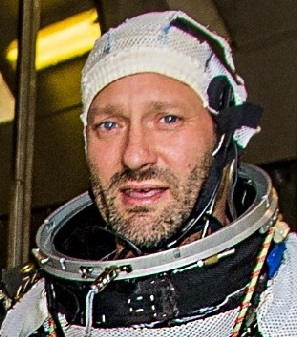
\includegraphics[width=100mm]{Interview_Figure_021}
	\centering
	\caption{Cameron M. Smith in self-made pressure suit
		{\normalfont\scriptsize \\ \copyright\ Cameron M. Smith, image used with permission
	}}
	\label{Interview_Figure_021}
\end{figure}

\begin{labeling}{IJSRA}
	\item[IJSRA (International Journal of Student Research in Archaeology)] \emph{How did you get drawn to space sciences?}

	\item[Cameron M. Smith (CMS)] I was a child of the Apollo generation, when people first walked on the Moon. Living in Texas, my Dad took me to the Houston Space Center. This was pre-terrorism and Dad was wearing a suit and looked like an engineer and we just walked the site freely, away from the tour. We met engineers in their offices. I was hooked when one showed me some of his math on a chalkboard. When we got home, Dad would check NASA films out via his university (he was a professor) and bring them home. He'd set up a projector in my room and I'd watch them over and over, 8mm film of the moon landings. Completely absorbing and engaging, I wanted to be there, to explore a whole world. From 10 - 14 years of age, then, I wrote to all NASA astronauts and some cosmonauts, and most replied, telling me how to get to space; stay in school; learn to fly; study hard. But by my mid-teens my eyes were losing perfect vision and I needed glasses; that nixed high-performance aviation, and subsequently I went into the human past, via archaeology, rather than the human future. That is, until the last decade, where a lot of renewed activity in space exploration has made room for me again, this time applying what we know of human evolution in the past to what will occur in the future as we begin to settle space, environments beyond Earth.

	\item[IJSRA] \emph{What, in your view, are some of the great challenges to future human space settlement, and how might these be overcome?}

	\item[CMS] This is exactly the sort of question I'm tackling in my forthcoming book, “Principles of Space Anthropology: Establishing a Science of Human Space Settlement” (Springer 2018).\footnote{\url{https://www.academia.edu/16883002/Principles_of_Space_Anthropology_Biological_and_Cultural_Evolution_Beyond_Earth}.} I am looking at human genetic and cultural adaptation, evaluating how ready we are, with these various adaptive tools, to take on space settlement. As a preview, you can see the précis of a paper I delivered at the Tennessee Valley Interstellar Workshop.\footnote{\url{https://www.academia.edu/33557172/The_Door_Stands_Open_Human_Biocultural_Adaptive_Strategies_are_Sufficient_for_Permanent_Human_Space_Settlement_and_Interstellar_Voyaging}.}

	\item[IJSRA] \emph{Please tell us more about your work.}

	\item[CMS] The essential issue is, how can we use what we have learned about human adaptation in the past to make more likely a success of the project of human space settlement. I think this project is of great significance in the history of Earth life; being able to live beyond Earth would constitute an important evolutionary transition and might well ensure that our species does not in the shorter term become extinct, a common fate in the history of species and of course the history of civilizations. These are the reasons that I think of space settlement not in terms of rockets and robots and gee-whiz technology, but a very human thing and even more importantly an extension of Earth life beyond the single planet. I have explored these issues in a semi-technical book, "Emigrating Beyond Earth" (Springer 2012); the preface is available online.\footnote{\url{https://www.academia.edu/2081591/Emigrating_Beyond_Earth_Human_Adaptation_and_Space_Colonization}.}

	\item[IJSRA] \emph{How might humanity evolve as a space-faring species?}

	\item[CMS] That is what I am investigating now. But generally it will be adaptation, both cultural and biological. We have a lot of experience with this in the history of our genus and species. The point is to build a science of human adaptation for space settlement. I am attempting to lay in this foundation.

	Humanity is right now exploring the idea of space settlement. This was the original goal of space pioneers such as Tsiolkovski—by the way, he drew pictures of families and communities in space long before space access became a supreme concern of federal governments and militaries. In the last two decades, though, private approaches to space access have rekindled the original concepts. Nothing we create begins without thought, so I am only being a little hyperbolic, I think, when I say that space settlement is beginning now. The question is, will this succeed? Because I think it is important—not just for humanity or civilization, but for the larger phenomenon of the evolution of Earth life—I am contributing what I can to make it more likely to succeed. Here's a bit of the preface to my forthcoming book 'Principles of Space Anthropology' (Springer 2018 or 2019) to explain exactly how:

	“In 1963, Siegfried J. Gerathewohl, NASA’s biotechnology chief, wrote... \emph{Principles of Bioastronautics}, outlining the need for this new field of study... At [that time] bioastronautics was established as a field with tight focus on individual human explorers, which was appropriate for its time. But today, plans include space settlement by populations, which raises many new issues; individual physiology is of course a different phenomenon than, say, population genetics, and individual psychology as short-term adaptation is different from cultural adaptation by reshaping behavioral norms in accordance with new circumstances. For these reasons, a new field of study—to advance and make more likely the success of human space settlement—is required. In this book I propose, describe, and outline the fields of space anthropology or exoanthropology... below I formally outline the need for space anthropology:

	Human space settlement will require novel biological and cultural arrangements unknown to current space exploration. These arrangements, guided as adaptations, will sustain human populations in environments—gravitational, radiation and chemical, for example—unfamiliar to the human adaptive suite after 100,000 years of modern human culture and biology on Earth. The new field of anthropology that studies such adaptive efforts is space anthropology or \emph{exo-anthropology}, exo- referring to beyond Earth, in the same way it is used in the term \emph{exobiology}.

	Specifically, I propose space anthropology to have three main functions:

	\begin{enumerate}

		\item To help specify the engineering problems to be faced by space planners concerned with space settlement by populations of humans and their domesticates, rather than space exploration by small crews and individuals.

		\item To evaluate the capacities of humanity’s various adaptive tools—cultural, biological and technological—to adapt to reasonably foreseeable space settlement plans, for example in Earth-orbital or Mars communities.

		\item To make recommendations that would assist in human adaptation to environments beyond Earth, particularly based on evaluations of human adaptive capacities identified in function 2.

	\end{enumerate}

	Space anthropology may be considered an anthropology applied to the specific goal of assisting in safeguarding the human hologenome, some of humanity’s most important domesticates and symbionts, and the totality of human knowledge, by the permanent settlement of human populations biologically and culturally independent of Earth.”

	\item[IJSRA] \emph{You're involved in developing better space suits. Can you tell us a little about what drives this innovation?}

	\item[CMS] Regarding the space suits, it is a way for me to materially participate in the human adaptation to space. The exploration and settlement of the Pacific by Lapita peoples three millennia ago was not done by sitting around and thinking about it, it was done by building and trying out physical objects, including sailing craft. I wanted that same material engagement. It's hard for me to describe my visceral frustration with the fact that just some tens of miles above our heads the atmosphere thins out and you have—the expanse of the universe to explore. I can't get there with my technology, and rockets remain too expensive, but with a high-altitude balloon and my suits I can get close, I can get a glimpse. And building the suits by hand is a fantastically rewarding challenge. There is a lot of frustration and a few very delicious and thrilling successes. Finally, the suit project has attracted interesting people who have become my friends. They have come to me asking about it, and then joined our effort. A lot of the work used to be solitary, but now I have friends who can help me with this dream, and I'm thankful for that. I've written about \num{10} books and that is a solitary profession in my experience, but also rewarding. So, having friends who share my dreams has been a very personal reason for the project as well.

\end{labeling}

\IJSRAseparator

\newpage

\IJSRAsection{Jim Pass, PhD}

Dr. Jim Pass is founder, CEO, and board member of the non-profit Astrosociology Research Institute (ARI), which finds its homepage at \href{<www.astrosociology.org>}{www.astrosociology.org}. He is Executive Editor of ARI’s \emph{Journal of Astrosociology}, and Associate Editor of the \emph{Astrosociological Insights} newsletter. Jim tweets at \href{<twitter.com/astrosociology>}{@astrosociology}.

%FIGURE 031: Jim Pass
\begin{figure}[!tb]
	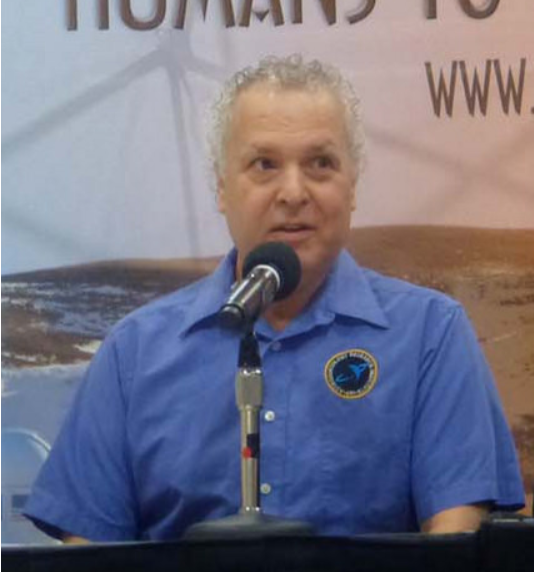
\includegraphics[width=100mm]{Interview_Figure_031}
	\centering
	\caption{Jim Pass at the Mars Society 20th Annual Convention, cropped from original at	\url{https://www.flickr.com/photos/mdrsphotos/37063952416/in/album-72157686333643733/}
		{\normalfont\scriptsize \\ \copyright\ Mars Society, image used with permission of Jim Pass
	}}
	\label{Interview_Figure_031}
\end{figure}

\begin{labeling}{IJSRA}
	\item[IJSRA (International Journal of Student Research in Archaeology)] \emph{First of all, what is \emph{astrosociology}?}

	\item[Jim Pass (JP)] Simply put, the study of \emph{astrosocial phenomena} (i.e., the social, cultural, and behavioral patterns related to outer space). As I will explain, I did not coin this term, but I had to put a definition to it. This proved to be a more difficult task than I first anticipated. In the course of a few months, this definition evolved into what I just stated. The difficulty of developing the actual definition of astrosocial phenomena was not the big problem. Rather, it was coming up with the concept of astrosocial phenomena itself, which was a strange process to me. This term is important because it is shorthand for the longer definition. It also serves to narrow the focus from all other social, cultural, and behavioral patterns that are not related to space, which also allows for contrasts and interactions between astrosocial and non-astrosocial sectors in society as well as between phenomena, forces, and so forth.

	\item[IJSRA] \emph{How did you get drawn to space scholarship?}

	\item[JP] Space has always interested me since I was younger than ten years old. I had a book on the solar system that my parents gave me, which by the way, certainly contained a great many inaccuracies—but it fascinated me. I kept abreast of the Mercury, Gemini, and Apollo programs through the news, books, newspapers, and periodicals the best I could. I was 13 years old in 1969 when Neil Armstrong first set foot on the Moon and I watched it on TV with fascination like almost everyone else around the world. Science fiction always played a large role, especially the various incarnations of Star Trek. All of these early influences placed a love for outer space in the back of my mind. I moved on to other things, but I ultimately came back to it with the founding of astrosociology as the final area of my career. I majored in criminal justice and sociology as an undergraduate. I went on to earn my Ph.D. in sociology at the University of Southern California with concentrations in criminology and political economy. When I graduated from USC in 1991, I had no idea that this return to outer space issues would occur even though apparently it had been incubating for decades. Over time, then, the space bug started to come to the surface, though the fact that I wanted to apply my sociology education to the study of space issues was a gradual realization that smacked me over the head one fateful day, which is described below. Prior to that momentous occasion, part of it was the fact that so many others were pursuing sociology subfields such as criminology, social inequality, family, and political economy—though these and all other important social-scientific topics relate to astrosocial phenomena. I guess I wanted to pursue something different, and hardly anyone was focusing on outer space within the sociology discipline. By the way, although astrosociology started out as what I thought of as a sociological subfield, it rather quickly became a multidisciplinary field based on inquiries from individuals in a number of different social and behavioral sciences, humanities, and even the arts. Therefore, the field expanded to include all three components of what I call the “other” branch of science, which exists in contrast to the natural and physical sciences including the STEM disciplines.

	\item[IJSRA] \emph{What does the Astrosociology Research Institute (ARI) do, and what prompted you to found the ARI?}

	\item[JP] Please allow me to answer the two parts of this question in reverse order. The fateful day occurred in late December of 2003: I came across an article on the Internet by Allen Tough who was also frustrated by the low number of social scientists focusing on outer space generally, and SETI (the Search for Extraterrestrial Intelligence) specifically. He suggested founding a new field and recommended “socio-astronomy” or “astrosociology.” When I read the latter term, it was like I was hit by lightning! The first thing I did was purchase the Astrosociology.com, Astrosociology.net, and Astrosociology.org domain names. From 2004-April 2008, I ran a small proprietorship called “Astrosociology.com” that introduced the proposed field of astrosociology to the world. In May 2008, once enough supporters of the field of astrosociology existed, I founded the non-profit organization ARI in conjunction with actually working on the Astrosociology.org website that I programmed myself without any training, which I admit is pretty evident. Thankfully, our website is finally in the midst of a professional upgrade. Thus, the founding of the ARI was actually just a continuation of the development of the field that expanded from me taking the lead to a non-profit organization with officers, board members, and advisors. I knew that we had to formalize the movement for it to gain additional legitimacy. A single-person front for a movement that I hoped would advance was not the best vehicle for development of a new academic field that I knew would face challenges. The establishment of ARI was a crucial step in astrosociology’s development. ARI’s existence is a testament to the fact that astrosociology is developing; that this field is moving in the right direction.

	ARI exists to facilitate the development of astrosociology as an academic field, which, again, is the study of \emph{astrosocial phenomena}. It is a non-profit organization that promotes and engages in astrosociological education and research. One of our major programs is called “Astrosociology in the Classroom,” which exists to place astrosociological content into schools, colleges, and universities. Although this has proven to be a bit difficult, recent progress in the form of greater recognition is quite frankly encouraging.

	ARI also puts out two major products that provide avenues for promoting astrosociological education and research, which is helpful to any academic field. The first is our newsletter \emph{Astrosociological Insights} which is an unrefereed publication (currently online-only). Articles are accepted or rejected, and edited, by our newsletter editors directly. It provides more of an informal place for individuals to report their work and ideas about astrosociological topics. Secondly, \emph{Journal of Astrosociology} (JOA) is a blind refereed online publication that involves higher standards of acceptance and content. We have a quite prestigious group of editors on our panel, which is quite satisfying. Both publications have resulted in a new period of growth and recognition while providing a way to increase membership in the community. All issues/volumes of each publication are available at this time at no charge at the astrosociology.org website.

	By the way, 2018 marks the tenth anniversary of ARI and we are planning events to coincide with this momentous occasion.

	\item[IJSRA] \emph{Please tell us more about your work.}

	\item[JP] Because ARI’s central mission is to develop astrosociology as an academic field, the focus on education and research describes my work in a general sense. My work basically consists of trying to find new ways to promote the development of astrosociology as a multidisciplinary academic field and getting new people involved. I write about different astrosociological issues in order to demonstrate the diversity of topics involved with the various astrosociological subfields. Examples include medical astrosociology, planetary defense, SETI, astrobiology, space law, space policy, science fiction, space art, and astrosociology research and education. A main message that I provide to people is that you do not need to be a rocket scientist to study space issues. The human dimension is just as important as the STEM-based issues and, in fact, they are two sides of the same coin characterized as space exploration and settlement. The increasing influences of astrosocial phenomena occur most obviously in space, of course, but also in terrestrial societies. Thus, they affect the daily social lives of Earthlings, which provides adequate reason in my mind to accelerate the inclusion of more social scientists, humanists, and artists in the study of space issues. Much greater collaboration is needed within each branch of science and between the two branches. I push for the convergence of the social sciences, humanities, and arts among those interested in space issues so that we can build the astrosociology community and an organized literature, and get astrosociology into the classroom (the latter of which is one of our flagship programs). Recruitment of new supporters and astrosociologists is also a key part of my work.

	I try to publish as much as I can and attend conferences. The Mars Society Convention is one example. Our Virtual Library page at \emph{Astrosociology.org} hosts a number of papers on various subfields to illustrate what astrosociology covers and why it is important. Most of the resources are available for free while some are publications in the form of chapters in books. Some of these I have written. On Twitter and Facebook and sometimes other social media, I write about astrosociological topics daily. I finally just surpassed 2,000 followers on Twitter, so there seems to be a general increase in the level of support for astrosociology. My followers are from diverse backgrounds, which I like because it reflects the field’s multidisciplinary aspect.

	As the CEO of ARI, I am constantly looking for collaborations with other individuals and entities that focus on space and see the value of the human dimension of space exploration and settlement. This is important for a couple of reasons that come to mind. First, many individuals conduct what one may term “astrosociological research” though they often do so in isolation or without a larger community in which to interact with others doing similar things. Secondly, organizations can work together pooling their resources and thus accomplish things that would be impossible on their own. The same is true of individuals who join the astrosociology community.

	%FIGURE 032: ARI
	\begin{figure}[!tb]
		
\includegraphics[width=60mm,scale=0.75]{Interview_Figure_032}
		\centering
		\caption{Astrosociology Research Institute logo
			{\normalfont\scriptsize \\ \copyright\ the Astrosociology Research Institute, image used with permission
		}}
		\label{Interview_Figure_032}
	\end{figure}

	\item[IJSRA] \emph{What, in your view, are some of the challenges currently facing astrosociology?}

	\item[JP] Probably the main challenge comes from the social science and humanities disciplines and fields. It is impossible to develop astrosociology to its full potential when there are no courses or programs for students. Ironically, those in the space-related STEM disciplines and fields are generally more receptive to astrosociology and collaborating than social scientists and humanists. Mainstream social scientists and humanists have historically ignored outer space and, in my experience, viewed related topics as fringe science because they often place astrosociological issues in the same camp as actual fringe sciences such as UFO abductions and astrology. Recruitment has become somewhat easier over the years, but the status quo still exists. In fact, I have received greater support overall from STEM disciplines than from social science and humanities disciplines. Luckily, social change is inevitable and so we are making strides in reaching out to the latter disciplines. I am convinced that students are our best hope.

	Like with all non-profit organizations that exist, fund raising is a difficult proposition. Asking for money for causes such as fighting diseases, disaster relief, and calls for religious support, while not a simple process, are generally less difficult than trying to promote a developing new academic field. On top of that, which cannot be overstated or mentioned too often, astrosociology is developing in a climate in which social scientists and humanists have largely ignored space issues for the bulk of the traditional space age, although great headway has occurred since we established the ARI in 2008. Then in 2011, we put together a special issue in the journal \emph{Astropolitics}. The result was increased recognition that astrosociology exists and more people expressed to us that such an academic field filled a void; that is, the human dimension of space exploration requires greater attention as the impact of astrosocial phenomena continues to increase. It was not like astrobiology’s much more rapid growth as an academic field, though it still serves as an important model demonstrating how a multidisciplinary field can develop. Moreover, the two fields interrelate in a number of different ways. For example, finding life elsewhere in the Milky Way solar system or beyond will have profound social, cultural, and behavioral implications.

	\item[IJSRA] \emph{Do you have any other stories to share about your experience in the field of space science?}

	\item[JP] In 2004, when I went to my first sociology conference to promote astrosociology, I was speaking with one of the organizers of the American Sociological Association (ASA) conference. When I mentioned astrosociology and its definition, her response was to roll her eyes and walk away. This reaction presented me with a personal version for some of the resistance I would soon encounter via email and on social media. The ASA has never accepted my proposals for an astrosociology session, though a couple of regional sociology associations in California did so early on. Interestingly, however, the ASA-SKAT (Science, Knowledge, and Technology) section published my submission entitled “Perspective: The Need and Relevance of Astrosociology as a Subdiscipline” in their newsletter. Additionally, Thomas Gangale and Marilyn Dudley-Flores supported me between 2004 and 2008, including writing conference papers about astrosociology. I met them at that ASA meeting in 2004 and they were the two other officers that signed on with me to create the ARI. They moved on soon after that, relinquishing their positions, but they were important contributors in the early days along with Dr. Albert A. Harrison. As mentioned, the space community has been more welcoming than the social science community, especially in the beginning. In particular, the American Institute of Aeronautics and Astronautics (AIAA) accommodated the idea of astrosociology since 2006 or so. In fact, most of my publications come from presentations at AIAA conferences. While this collaboration is vital, we at ARI are making concerted efforts to also collaborate more with the social sciences and humanities. There are many individuals and even some programs and departments dealing with astrosociological-like topics, but mainstream social scientists and humanists tend to view space as less than interesting or irrelevant to everyday social life. We need to change such attitudes, and we are trying.

	In the early days of astrosociology’s development, an extraordinary thing occurred along with the backing of Thomas Gangale and Marilyn Dudley-Flores amidst a somewhat troubling negative atmosphere. Dr. Albert A. Harrison came along and strongly supported me in my effort to develop astrosociology starting in 2005. He provided legitimacy to a nascent academic field that enjoyed very little support at the time. Of importance, Dr. Harrison was a social scientist who studied planetary defense, SETI and astrobiology, among other topics. ARI was not founded until 2008, so his support of the field was based mostly on my professional relationship with him. And, in fact, he was the first to join our Board of Advisors in 2008. Unfortunately, Dr. Harrison passed away much too soon in 2015. For anyone interested in astrosociology, his works are a fantastic wealth of information. I used to joke with him that he was doing astrosociology before I founded the field in 2004.\footnote{A listing of his publications is available at \href{http://www.astrosociology.org/AAH-InMemoriam.html}{www.astrosociology.org/AAH-InMemoriam.html}, some of which are available at ARI’s \href{<www.astrosociology.org/vlibrary.html>}{Virtual Library}. One of the publications, by Dr. Pass is a tribute to Dr. Harrison: \href{<http://www.astrosociology.org/Library/PDF/Space2016-JPass-AlbertAHarrison.pdf>}{www.astrosociology.org/Library/PDF/Space2016-JPass-AlbertAHarrison.pdf}.}

	I must also mention Christopher Hearsey, who initially served as an officer for ARI and later became Editor-in-Chief of the \emph{Journal of Astrosociology}. He also served as our Chairman of the Board. He resigned in December of 2017 to run for Congress. His work with ARI provided a stability and direction since 2009 or so that helped me in collaboration with him to move forward more forcefully in the development of astrosociology as an academic field. He served as the editor on the special issue of \emph{Astropolitics} mentioned earlier that is dedicated to astrosociology. That gave ARI added recognition and legitimacy. His counsel and hard work has put our non-profit organization in a great position moving forward. Kathleen Toerpe, Renato Rivera Rusca, Simone Caroti, Geoffrey Notkin, and the members of our Advisory Board and editors of \emph{The Journal of Astrosociology} all contribute to the ongoing development of astrosociology. Dr.~Toerpe, the original editor, made our newsletter a great success. Finally, Dr.~Michael Dodge, Assistant Professor and Director of Space Studies at the University of North Dakota, has taken over Christopher Hearsey’s duties as Board Chairperson, ARI Officer, and editor of our newsletter and journal. He is doing a great job assuming such a heavy load.

	Between 2009 and 2011, ARI hosted the Astrosociology Symposium, which was part of the larger Space Propulsion and Energy Sciences International Forum (SPESIF). Each of the three symposiums focused on astrosociological issues and some of the papers presented were published. While the SPESIF conference folded after 2011, it provided ARI with an additional opportunity to get more people involved and grow the community. It also provided greater publicity for the very existence of astrosociology and the developmental work ARI was conducting. This provided additional legitimacy to the both our organization and the academic field.

	Additionally, and quite relevant to this interview, Alice Gorman, “Dr. Space Junk,” recently joined ARI’s Board of Advisors. She is leading the way in the field of space archaeology! As a multidisciplinary endeavour, ARI continues to welcome diverse individuals to contribute to the development of astrosociology.

	Volume two of the \emph{Journal of Astrosociology} was published in 2017, which brings social-scientific analysis to space topics traditionally covered by physical and natural scientists and STEM individuals, and the Call for Articles for volume three is currently available on our Journal page at \emph{Astrosociology.org}. Additionally, the latest issue of our newsletter that focuses on space law and policy is now available at our website.\footnote{\url{http://astrosociology.org/Library/PDF/Newsletters/ARI-Newsletter_Vol-6_Iss-1-2017.pdf}} The next issue’s Call for Articles is also available. The topic is “the impact of the space arts on societies.”

	We are working daily to advance the development of astrosociology.

\end{labeling}

\IJSRAseparator

\IJSRAsection{Keirsten Snover, MA}

Keirsten Snover is the founder of Space Anthropology Services, with its homepage at \href{www.spaceanthropologyservices.org}{www.spaceanthropologyservices.org}. \emph{Please note: As of March 2018, Keirsten Snover is no longer active as an anthropologist due to the progression of a neuromuscular disease to advanced stages. The Space Anthropology Services website, blog, and all associated social media accounts are no longer active.}

	%FIGURE 041: Keirsten Snover
\begin{figure}[!tb]
%	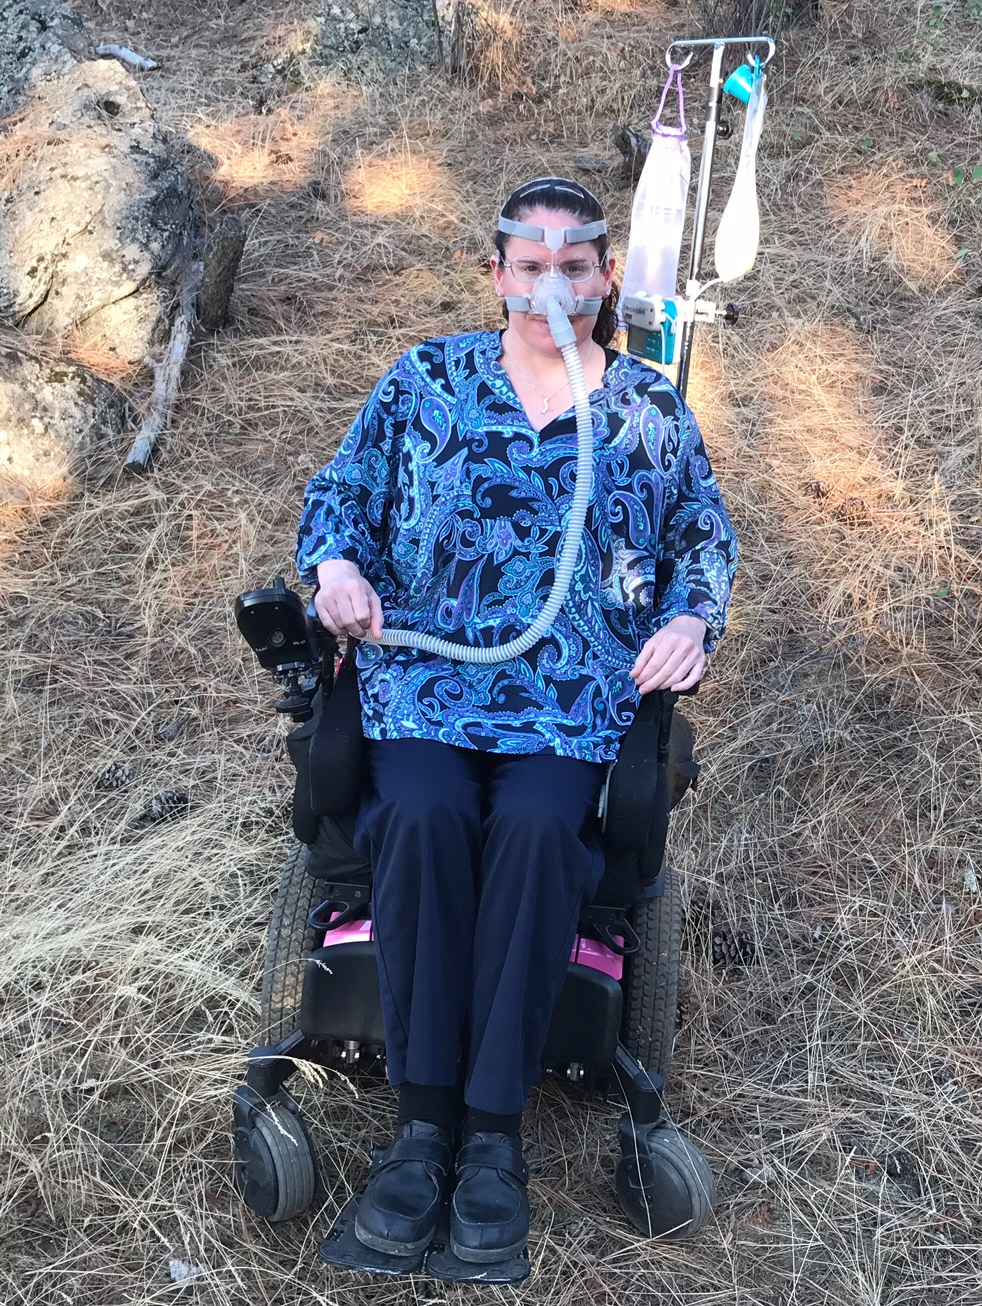
\includegraphics[width=.5\linewidth]{Interview_Figure_041}
	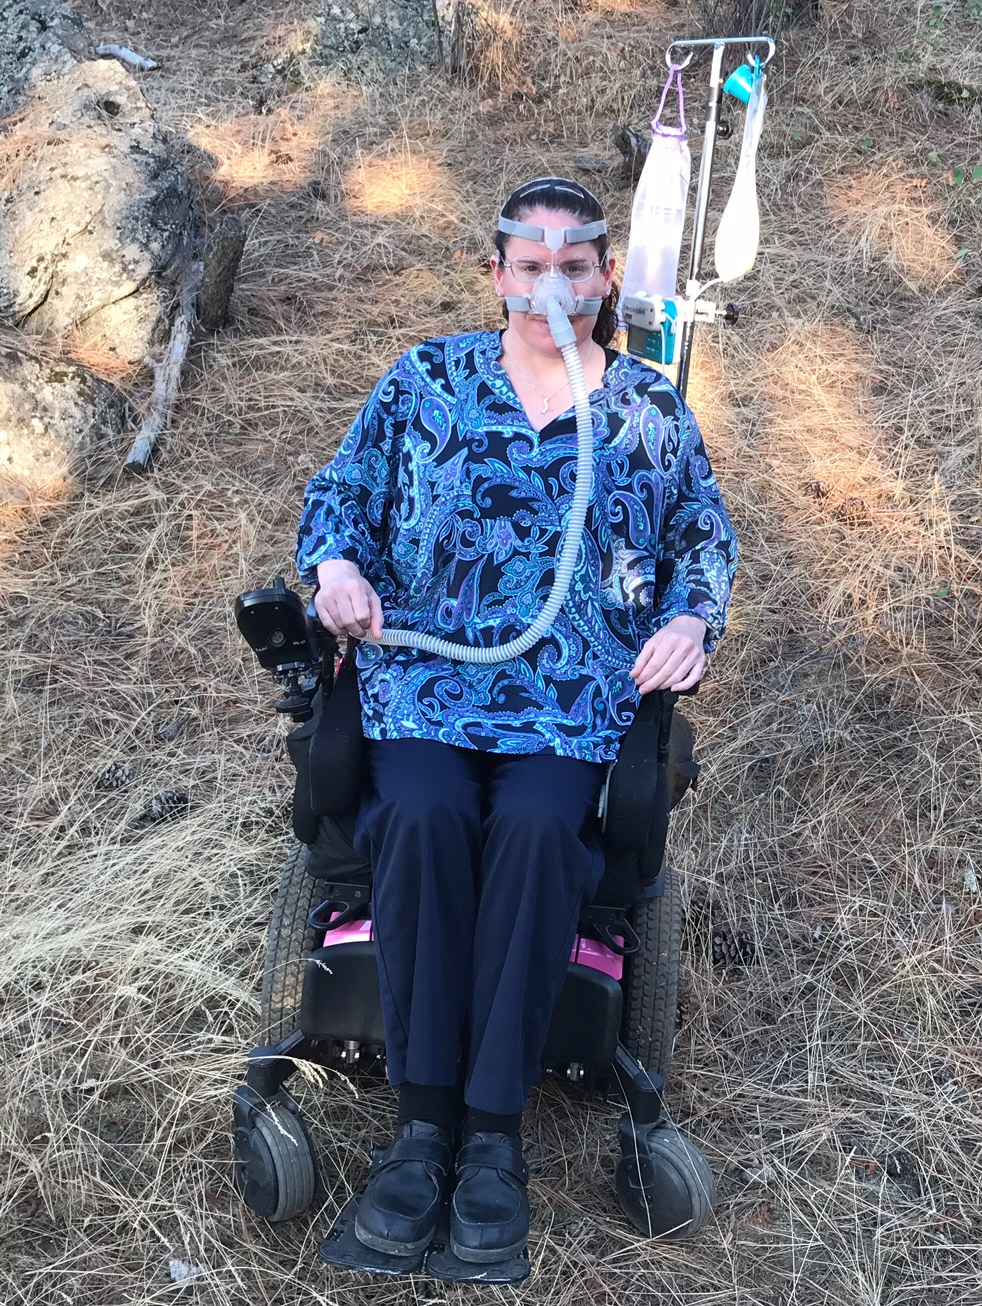
\includegraphics[width=100mm]{Interview_Figure_041}
	\centering
	\caption{Keirsten Snover
		{\normalfont\scriptsize \\ \copyright\ Keirsten Snover, image used with permission
	}}
	\label{Interview_Figure_041}
\end{figure}

\begin{labeling}{IJSRA}
	\item[IJSRA (International Journal of Student Research in Archaeology)] \emph{How did you get drawn to space scholarship and education?}

	\item[Keirsten Snover (KS)] The study of space is a fairly recent endeavor for me. I started studying anthropology, mainly medical anthropology, focusing on how people in different cultures respond to different diseases and their related health knowledge, attitudes, and practices. I was very interested in how people perceive disease, and how that perception then affects health-seeking behaviors. This focus eventually led to a research position at the Cleveland Clinic in Cleveland, Ohio, where I was involved with a project looking at perceptions relating to genetic diseases. My change to space scholarship started when I discovered (while doing medical research in the hospital’s library) that the Cleveland Clinic had a Center for Space Medicine. I had never heard of the field of space medicine, but as a medical anthropologist I was intrigued! As I investigated further, I found that the Cleveland Clinic Center for Space Medicine had been created to work with the nearby NASA Glenn Research Center on research related to health problems encountered in space. It didn’t take too much additional research before I realized that space medicine was a potential field for a medical anthropologist like me to pursue, and so after my position at the Cleveland Clinic was over, I signed up for graduate-level coursework in space science. It was during this coursework that I realized there was more connecting space and anthropology than just the area of space medicine. The more areas of space science I learned about, the more ways I saw that anthropology could contribute. I brought up this topic with several space scientists at a NASA conference that I attended, and the scientists agreed, and so my decision to study space was solidified.

	Growing up, I was one of those kids who made spaceships out of empty boxes, wondered about life on other planets as I looked at the stars at night, and obsessively watched Star Trek. But I never really saw space as a field to study. When I was considering college majors in high school, I knew I had a long-standing interest in all sciences, but I had no idea that you could study topics related to space beyond the field of astronomy. I wasn’t really interested in making a career out of using telescopes, or studying the rings of Saturn. I was more interested in human space exploration, and if we would ever visit or live on other planets, but this was only science fiction back then. Unfortunately, when I was growing up I wasn’t really exposed to female role models in science, let alone in the space sciences. Even though I was in elementary school when Sally Ride was flying to space with NASA, I didn’t view involvement in space as something that women did, or that I could do someday myself. For years, I faced a lot of pressure when I told people that I wanted to be a research scientist—I was constantly encouraged to become a school teacher or nurse instead, and to follow a more traditional female career path. For kids growing up today, things are very different. There is much more exposure to female role models in the different disciplines of science, and girls are actively encouraged to pursue STEM fields. This movement is something I strongly support, and my childhood experiences have significantly influenced my desire to be involved in STEM education. In addition, my childhood dream of becoming a research scientist was initially nurtured by a middle school science teacher who helped me design research projects and compete in local science fairs. I hope that by becoming involved in educational outreach, I can “pay it forward,” and encourage other young students interested in science to pursue their dreams, too.

	\item[IJSRA] \emph{What can anthropologists uniquely contribute to space ventures?}

	\item[KS] It seems every time I tell people that I am an anthropologist who studies space, people become rather confused (even other anthropologists). When I then provide a short example or two about how anthropology can contribute to the study of space, I tend to get the same reaction over and over, “Ohhhh. I guess all you need now is a space program!” There are two important things to take away from this type of response. First, that it may not be obvious, even to other anthropologists, what our discipline can contribute to the space sciences. Second, not everyone is aware there is a current space program, or that numerous countries around the globe have their own space programs. More awareness is needed, for anthropologists and the public, regarding space in general and the role all social scientists can have in the space sphere. In addition, more awareness is needed among members of the “hard science” space community that collaboration with social scientists can be beneficial.

	So, what can an anthropologist contribute? For me, asking for a list of ways that anthropology can contribute to space is similar to asking what you can do with a degree in anthropology. What can’t you do with a degree in anthropology? There are numerous topics in the space realm that an anthropologist can study. It seems the more one becomes immersed in the study of space, the more potential research areas become evident. So, I feel a better question is, “What topics in space science can’t anthropology contribute to?” Space topics of potential interest to anthropologists include everything from how the human body reacts in low gravity conditions, to the practice of flying artifacts (like a Clovis point) into space, to the controversial building of huge telescopes on land sacred to Native populations. I highly recommend reading the ARI's “List of Suggested Topics” for their journal.

	There are many research ideas anthropologists could examine within the topic of space settlements. Currently, multiple space companies in various countries are planning lunar bases and/or settlements on Mars. This process involves the creation of small societies, often comprised of culturally diverse international teams. Anthropologists are experts in small societies as well as cultural diversity, so this is an important research area. All the aspects of Earth-based societies that anthropologists have historically studied will likely surface in space societies—for example, issues of language, food, culture, division of labor, politics, death, social constructions of law, health and illness, and cross-cultural communication. Anthropologists could consider whether the significant anthropological literature on these topics can be useful in the creation and maintenance of small societies in space.

	Besides the basic operations of space societies, there are potential research questions relating to the effects of living in a space settlement. For example, how will people adapt culturally and physically to living in a space habitat? Can we learn anything from anthropological literature regarding humans living in extreme environments here on Earth? Studying the life of astronauts aboard the International Space Station and in terrestrial analogue communities (simulated space settlements in isolated places on Earth) may also be helpful (and also are interesting topics of study themselves as they, too, are small societies). In addition, there are questions at the intersection of human identity and living in space, involving symbolism, meaning, cognitive maps, and more. For example, what does it mean to be a human who does not live on our planet? What will Earth mean to humans born on the Moon, Mars, or elsewhere? The rise of the “Mars Generation,”—young people around the world publicly dedicating their lives to pursing their future on another planet—is also a fascinating phenomenon relating to human identity and space worthy of anthropological study.

	Another area of research potential surrounds who can travel to space, whether as a space tourist or new member of a space community. Astronaut selection has been critiqued in the past for its lack of gender and cultural diversity. Will future members of space societies reflect the diversity of humans on our home planet? Concerns also exist about the relationship between economics and access to space. Will most space tourists only be composed of wealthy individuals who can afford to pay for a ticket to the Moon or Mars? Will attainment of a certain educational level be a prerequisite to acceptance as a member of a new space society? What implications will result from restrictions on who can go to space or live in space? These specific questions of human access to living in and visiting outer space may be relatively new, but the basic underpinnings are similar to research questions anthropologists have asked on Earth many times before in other situations.

	\item[IJSRA] \emph{Why is education about space important, and what are some ways you have engaged in science communication?}

	\item[KS] A couple of years ago, I was attending a special event sponsored by the NASA Glenn Research Center for the 25th Anniversary of the Hubble Space Telescope in Cleveland, Ohio. During one portion of the event, an auditorium was filled with members of the local public and school children from multiple schools. After an inspiring presentation about the Hubble Space Telescope, a question and answer session was offered. While I did not formally record and analyze the questions, it seemed the biggest question on many attendees’ minds consisted of different variations of “When is NASA starting up a space program again?” The NASA representatives seemed a little surprised by these questions, and in turn many members of the audience seemed surprised to hear that NASA had a current operating space program and always had one. What I found most interesting was that this was happening in a city with a NASA research center that frequently engages in community outreach. This made me wonder what the level of space science-related knowledge was in cities that did not have the benefit of a NASA center or other major space-related resource nearby.

	Over the past few years, I have consistently encountered people from all walks of life who are not aware of the tremendous developments occurring in the space sciences. There also seems to be little awareness among the people I spoke with about significant human achievements relating to space, such as landing on a comet, the mission in progress to land on an asteroid, finding liquid water on Mars, and new images of Pluto. As an anthropologist, I realize this is likely the result of the interaction of multiple complex social, cultural, educational, economic, and political factors. However, this experience (and other similar experiences) prompted me to consider the larger question of the general public’s access to resources, specifically information about space and space exploration. It was then that I realized that perhaps I should be involved in educational programs about space. I think that education about space is important because being involved in outer space provides access to resources, like technology spin-offs, economic development, scientific advancement, international cooperation, and more. Currently, this access is not distributed equally throughout our world—developing nations do not have the same amount of access to space as developed nations, and even within developed nations access to space is uneven among citizens. Many space-related organizations have stated that outer space is for everyone, and I strongly support this view. For me, the most important reason for space education is not necessarily the specific space-related knowledge imparted, but helping provide more equal access to that knowledge, which can then help provide more equal access to the resources of space.

	As part of this, I have been engaging in science communication efforts, mainly through online interaction. A few years ago, as a part-time project I started an organization called \emph{Space Anthropology Services}. While my original vision was much broader, right now it is focused on promoting the intersection of space and anthropology through a website, blog, Facebook page, and Twitter. Besides providing related content, I also interact one-on-one with people from around the world, and answer various questions about space and anthropology that are sent to me through these online channels. In addition, I have created educational infographic posters for past World Anthropology Days, which help illustrate some of the ways that anthropology can contribute to the space sciences. I have also recently started engaging in more face-to-face science communication as well, through space-related presentations and workshops. In the past, I have provided several different anthropology workshops, including simulated archaeology dig workshops and forensic anthropology workshops. I found these to be very rewarding and well-received by attendees, and so I want to do something similar by providing workshops in the area of anthropology and space. As one example, I gave educational workshops about the recent solar eclipse, and passed out solar eclipse glasses provided by The Planetary Society. Some science communication projects currently in progress include the creation of online courses and involvement with other outreach organizations (such as NASA’s various Ambassador programs).

	\item[IJSRA] \emph{Please tell us more about your work.}

	\item[KS] My work in the field of space and anthropology is comprised of three major parts: research in the field of space anthropology, collaborative work with other scientists and organizations, and science communication. Previously, my research was focused mainly on anthropological contributions to space settlements. While this topic is still of great interest to me, I have decided to start focusing on the phenomenon of private citizens working on going to space with the hopes of living somewhere besides planet Earth. A few examples of this phenomenon can be seen with the space nation of Asgardia, Space Citizens, Space Nation, and The Mars Generation.

	Asgardia is an international project with the goal of creating a new nation in space. Hundreds of thousands of people across the world have submitted applications for citizenship, and are now working together to figure out the details of their new society, including everything from drafting a constitution to deciding on national holidays. Space Citizens is open to international membership, and the plans include building habitats in space and mining space resources. This project emphasizes that everyone in the world should have the chance to help create space settlements, regardless of income, religion, or disabilities. Space Citizens encourages the participation of those who don’t have formal training or degrees in the space sciences, and recognizes that everyone has a part to play. Space Nation has developed an Astronaut Experience Program and will soon be launching the first free global astronaut training program via a smartphone app. Each year, some of those who participate in the app-based training program will be selected to attend a filmed bootcamp, and the winner will be sent to space. Space Nation aims to bring space into our everyday lives, while promoting space education and wellness. The Mars Generation is both an organization founded by a young aspiring astronaut, and an identity used by young people who want to go to space (even if they are not formally affiliated with the organization). It is the children of today who will likely become the ones able to live on Mars, hence the name “The Mars Generation.” The children and teens who identify with this are actively preparing themselves to be the best candidates to travel to Mars, through various activities such as earning SCUBA and pilot license certification, attending space camps and other training programs, and learning other languages. In addition to the four described, there are other citizen-based space endeavors, and I look forward to further research on this topic, including participant observation with some of these programs.

	In addition to research, I am collaborating with other scientists and organizations. For example, I am working with NanoApps Medical, Inc., on projects involving nanotechnology. This company is working on developing terrestrial nanomedicine to the point where a Global Health Care Equivalency is reached, meaning that every person around the world has access to the same nanomedical diagnostic and therapeutic technologies. In addition, NanoApps Medical is working on the applications of nanotechnology to space, especially in the field of nanomedicine. As a medical anthropologist who is also interested in space, these topics of nanomedicine, access to healthcare around the world, and applications of nanotechnology to space are of great interest.

	As previously mentioned, I am involved in science communication, and I’m currently working on several projects in this area. I am continuing to create space-related workshops for the general public, as well as online courses in the area of space anthropology. My biggest science communication project, still in the initial planning stages, is an educational space-themed event designed for people with disabilities. Sometimes people with disabilities can feel left out because they are unable to participate fully in some public events, so this event will have activities adapted for different kinds of disabilities. Also, many companies are finally realizing that hiring employees with disabilities is a good strategy for their business, and this includes companies in the space sector. At this event, I am envisioning a huge room like a gymnasium or conference center filled with different interactive activity stations. Each station will have a space-themed activity that can accommodate different disabilities. I'm thinking things like 3D-printed Moons so that attendees with visual disabilities can feel the craters. A station where you can listen to recordings of the sounds of space. An area with a simulated Martian landscape where people can drive power wheelchair "Martian rovers" over the surface. There will also be exhibits highlighting people with disabilities who work in space-related jobs. It is a big project, of course, but I’m very excited about it!

	\item[IJSRA] \emph{Do you have any other stories to share about your experiences in the field?}

	\item[KS] One of the field experiences that made a significant impact on me was when I went with a group of archaeologists to examine a rockshelter in the Channeled Scablands of Washington state. I vividly remember climbing up the hillside to the rockshelter, and standing inside the entrance. I looked out onto the shrub-steppe landscape, dotted with fragrant sagebrush, lavender-colored bitterroot flowers, and rock outcroppings. This view was picturesquely framed on three sides by the jagged basalt rocks forming the mouth of the rockshelter. It was a moving experience, not just because it was strikingly beautiful, but to stand there and realize that other humans may have taken shelter in the same spot as long as 10,000 years ago. I stood inside the rockshelter imagining what it must have been like for those humans, and felt a sense of awe that I can clearly remember today, many years later. I’m not completely sure what caused my reaction. This wasn’t my first archaeological experience—I had excavated archaeological sites before, and handled artifacts that were thousands of years old in the lab of an archaeology company that I worked for during graduate school. However, something about being in this rockshelter moved me in a way that hadn’t happened during my other archaeological fieldwork experiences. Perhaps it had something to do with the immersive nature of the experience, since I could see and feel the rockshelter above me, below me, and on all sides. Even now, I can distinctly recall the feeling of immense awe, and the same feeling can be re-created in certain circumstances. Have you ever seen space-related artwork that shows a person standing inside a structure on another planet, and gazing out across the barren landscape of the Moon or Mars? This seems to be a rather common theme in artwork related to space exploration. I enjoy looking at these images and imagining what it would be like to actually be in a space habitat, viewing the landscape of another planet in person. The feeling I get from this is very similar to the feeling of awe I had viewing the Channeled Scabland landscape from the rockshelter. Maybe one day, humans will live on Mars, and look out across the Martian landscape from a window on their home, all the while wondering what it was like to look out a window and see the landscape of planet Earth.

\end{labeling}

\IJSRAseparator

\IJSRAsection{Michael P. Oman-Reagan, PhD candidate}

Michael P. Oman-Reagan is a PhD candidate and Vanier Scholar at Memorial University of Newfoundland. In addition to journal articles, he writes for a variety of online publications including \emph{The Conversation} and \emph{SAPIENS}. His most recent paper is “\href{<https://arxiv.org/abs/1708.05318>}{Visions of Human Futures in Space and SETI}” with astrophysicist Dr. Jason T. Wright published in the \emph{International Journal of Astrobiology} and posted as a preprint to the arXiv. His work can be found at \href{<http://michaelomanreagan.net>}{http://michaelomanreagan.net}. Michael tweets at \href{<twitter.com/OmanReagan>}{@OmanReagan}.

%FIGURE 051: Michael P. Oman-Reagan
\begin{figure}[!tb]
	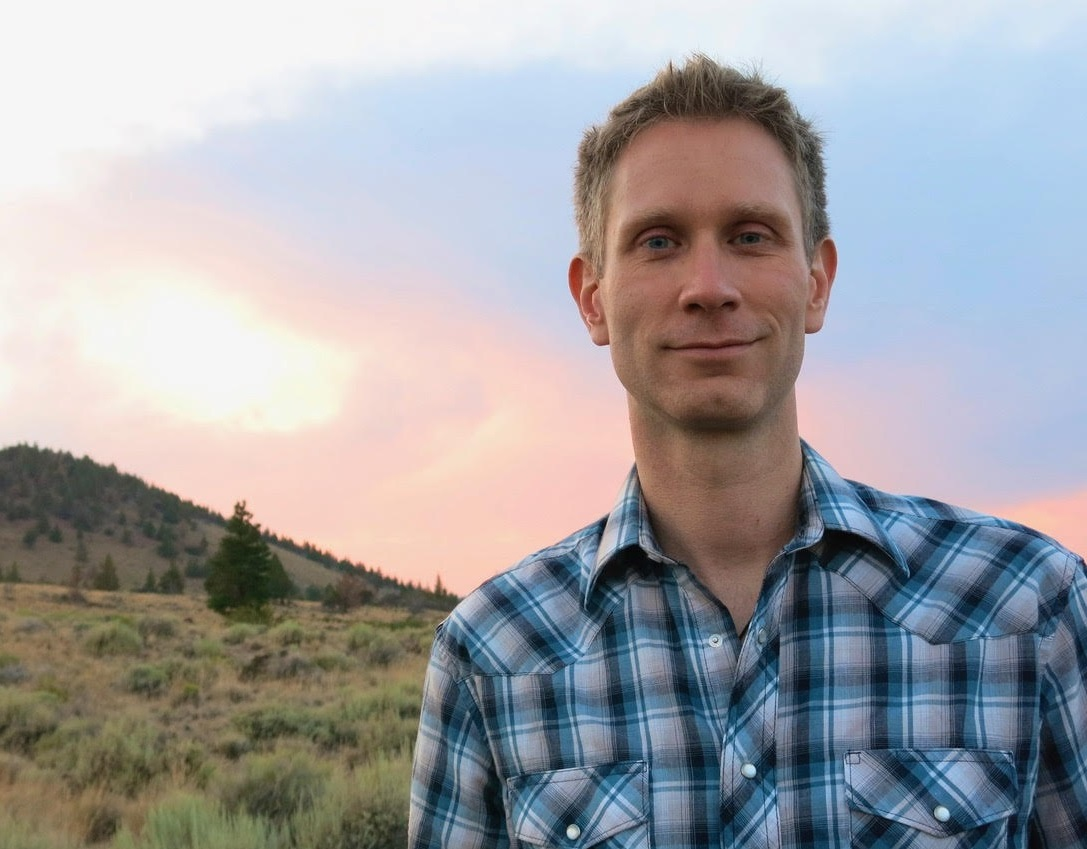
\includegraphics[width=100mm]{Interview_Figure_051}
	\centering
	\caption{Michael P. Oman-Reagan
		{\normalfont\scriptsize \\ \copyright\ Michael P. Oman-Reagan, image used with permission
	}}
	\label{Interview_Figure_051}
\end{figure}

\begin{labeling}{IJSRA}
	\item[IJSRA (International Journal of Student Research in Archaeology)] \emph{How did you get drawn to space science?}

	\item[Michael P. Oman-Reagan (MO-R)] Space has been on my mind since I was a child growing up in the rural west. The sky there was clear, with very little light pollution (or “skyglow”). Now, though, the Milky Way is hidden from one-third of humanity because of light pollution. I spent many nights on the roof looking up into the stars and into our galaxy during the summer—wondering what was out there, thinking about how looking into the deep universe speaks to what it is to be human here on Earth. I was a fan of science fiction as well, reading Heinlein, Asimov, Bradbury, Herbert, and all the classics, as well as science fiction media like Star Trek and Doctor Who. To me, these visions of other worlds and ideas demonstrated possibility, and reminded me that \emph{how things are} is not \emph{how they have to be}.

	I started out my academic career, however, as a biology major. I intended to study marine mammal socialization and intelligence, but I soon realized that my interests were broader than the scope of biology at the time, so I moved to philosophy where I could ask bigger questions about what these ideas of socialization and intelligence mean to us. From philosophy I moved to the secular, academic study of religion for more insight into the stories that humanity tells about the big questions: where do we come from? why are we here? So my first undergraduate degree was in religion, then I added anthropology because I wanted new methods to move outside of the text and into the world, using ethnography, participant observation and other techniques. Anthropology, as it was taught at CUNY, was a good fit because it allowed me to ask all of the questions I could ask in biology, philosophy, and religious studies, and add new areas as well. The anthropology I’ve been trained in has continued to be very interdisciplinary, easily citing other fields, writing experimentally, creatively, challenging the history of our discipline as well as disciplinary boundaries.

	My Masters work in anthropology was at Hunter College where I studied the intersections of activism and technology, looking specifically at transnational social movements. At the core, this research was about how we imagine better possible futures, and work to get there. My work on space science is motivated by the same questions about the future—about how we think about possibility, other worlds, the forms that life, culture, and society might take in space. Whether that’s humanity moving into space, or life that may already be out there.

	\item[IJSRA] \emph{What might human experience on Earth hint about future human life in space or on other planets?}

	\item[MO-R] Long before colonialism, humanity moved across our planet, adapting to new environments and challenges. Our species has developed a diversity of incredible tools: culture, language, religion, practice, stories, and all kinds of material and social technologies. All this diversity is precisely what could make us well-suited to moving into space, if we can do the work required here on Earth first.

	We have the tools we need to survive in space, but so far we’re not using them. I’ve been talking about these tools as the “cultural infrastructure” we need to move into space—this includes treating our environment as precious, because habitability has to be a priority in space. Cultural infrastructure also includes different languages, traditions, religions, philosophies. It’s all the diverse perspectives and approaches that have allowed us to survive on Earth. It includes ancestral and traditional knowledge, science, arts, humanities education—it includes healthcare as a right—and it includes mutual aid. We need to become a society that will always help anyone who needs our help. If we don’t adopt these as fundamental values and principles of a planetary society, we won’t survive in space, on the moon, or on Mars.

	So, to ensure a good future in space, we have to start here by looking at human history—we have to build on the success of that diversity here and do it collaboratively on a global scale. Then we will have the preconditions necessary for inclusive and equitable futures in space.

	\item[IJSRA] \emph{What are some of the challenges in doing space science research, and how can these be overcome?}

	\item[MO-R] One approach to studying space science might be studying scientists as “research subjects”—but as I’ve been doing my fieldwork over the last year I’ve found that it’s more productive and interesting for me to approach space scientists as colleagues. When I studied the Occupy movement in New York City, and activism in Indonesia, I joined those communities as a fellow activist, in solidarity. So I’m working to do something very similar with space scientists. As a result, I’m submitting white papers proposing ways that anthropology can contribute to interdisciplinary space science, and I’m co-authoring with astronomers. Joining the interdisciplinary space science world as an anthropologist is challenging because it it's not immediately obvious to many what anthropology can contribute—but I’ve found the community to be extremely welcoming. Another challenge is how you do fieldwork with communities that only come together during conferences. This kind of science-focused multi-sited work doesn’t offer what we traditionally think of as a field site, or even a laboratory like other sciences might. As a result, it takes much longer to join the community, to build rapport, and to collect data than if there was one location to visit and spend time in. These challenges demonstrate how important it is for departments and federal agencies to provide long-term funding and flexibility to researchers who take on these sorts of projects. It would be impossible for me to do the fieldwork I’m doing without the support of my department at Memorial University, the Vanier Canada Graduate Scholarship, and the Social Sciences and Humanities Research Council of Canada.

	\item[IJSRA] \emph{Please tell us more about your work.}

	\item[MO-R] My current research project is about engaging as an anthropologist with communities and groups who work on exploration beyond our solar system. I tend to call it “interstellar exploration” as a shorthand but it also includes exploration beyond the interstellar, to the intergalactic, and further.

	For my fieldwork I’m working with space scientists in Canada and the United States who explore beyond our solar system. I’m interested in three primary modes of exploration: observation, communication, and travel. Observation includes astronomers here in British Columbia who use instruments to look out into the universe to collect data. Communication involves researchers in the field of SETI (the Search for Extraterrestrial Intelligence) who listen for signals and consider sending them, mostly around the San Francisco Bay Area. Travel is about actually going there, whether through un-crewed spacecraft and probes like Voyager or through imagining and planning for a generation ship with a human crew to travel to another star.

	By looking at these interstellar exploration efforts as well as science-fiction and the history of space science, I’m trying to understand how we imagine the space beyond our solar system, what role it plays in imagining and creating possibilities for life, culture, society, politics, and more here on Earth and in the future in space.

	\item[IJSRA] \emph{Do you have any other stories to share about your experience in the space sciences?}

	\item[MO-R] Unlike us stuffier socio-cultural anthropologists it turns out that astrobiologists—much like archaeologists—throw great parties. And they really know how to have fun at conferences. The highlight of my fieldwork at AbSciCon (Astrobiology Science Conference) in Arizona this year was the open-mic night where astrobiologists sang songs about alien life, read science fiction stories, and more.

	\item[IJSRA] \emph{You are engaged in activism related to anthropology on social media, particularly Twitter. What prompted you to get involved? Should academia encourage, support, and/or reward activism?}

	\item[MO-R] I’ve been an activist since I was a teenager, and it’s something that comes out of necessity. In high school I watched as the news reported on murders of LGBTQIA people, and saw my classmates celebrated for publicly expressing that I shouldn’t have basic human rights. I wondered every day if someone would come for me next because of who I am. So for me it’s about survival, not only for me but for anyone who lives with this kind of bigotry and oppression anywhere in the world.

	Even if someone doesn’t have a personal experience of oppression, academics especially have an obligation to be activists. We live on a planet where a few people in power use violence to take resources from the rest, where we could feed, clothe, and house every human but we don’t. I think when it comes to academia the question should be: How can anyone look at the world we live in and not be an activist for social justice? We should really be asking about those with power, working in the management and administration of academic institutions, who ostensibly know so much about the origins and causes of inequality, structural racism, and bigotry and yet remain silent. In anthropology, I believe we have a special responsibility to speak out because our discipline has been complicit in colonialism, in writing racist narratives about civilization and cultural change, and in much of the pseudo-science around race that continues to be used in the public sphere. Although we often address that in our courses and teach our students about it, these ideas remain powerful outside of academia, often adopted as “common sense” notions about race and cultural differences. It’s our obligation as anthropologists to constantly work against the validation of those ideas and point out that the very discipline that created them has (mostly) long since abandoned them.

	Universities do have an obligation to support faculty, students, and staff in their activism for justice. At the very least by defending their academic freedom, and broader freedom and rights as human beings, and further by understanding that activism and public scholarship is a form of necessary labour. When we bring anthropological perspectives into the public sphere to address important issues of the day, we are also doing the work of demonstrating why our discipline is relevant. The work we do in writing for general audiences, conducting outreach, and public scholarship should be taken into account for students working toward degrees and for faculty working toward tenure. That isn’t to say it should be required of everyone because it does have a cost, but simply acknowledged as one of many possible legitimate paths and methods of engaging in scholarship and research, and of having “impact."

	Neutrality is an interesting claim, but it’s also a political claim which I’d argue isn’t itself neutral. I hope all the sub-disciplines of anthropology agree by now that there is no “view from nowhere.” I believe we must have the courage to take a side. Each time we demonstrate that courage, we show everyone around us that it’s possible. Speaking out for justice isn’t easy, it often has a cost—but the best way to address that cost is not to back down but to stand in solidarity with others who are also standing for justice. This is where many US universities have recently failed by not standing with their faculty and instead falling for the tactic of right-wing extremists who manufacture insincere outrage with the goal of punishing faculty who speak out for justice.

	\item[IJSRA] \emph{When inhabitation of space and other worlds becomes a reality, what roles do you envision of anthropologists and archaeologists? What lessons from life on Earth cannot be ignored?}

	\item[MO-R] Just as we’ve adapted our discipline to studying life in online and virtual worlds, and society and culture of other new digital technologies, anthropology and archaeology are already adapting to study human interactions with space. This will continue, with some interesting consequences. One day we might have anthropologists trained on the Moon, Mars, or a space habitat who come to Earth to do fieldwork. I suspect it won’t take long for human societies on other worlds, the cultures, practices, stories, habits, languages, and more to become quite different in ways that we’re very unlikely to be able to predict. In ways that may or may not be similar to the kinds of differences that emerged as humans have moved around the Earth.

	Looking far into the future, I also believe that anthropology is especially well suited to become the discipline that studies the non-human cultures of other worlds. Part of what I’m doing now is working on ways that anthropology can participate in the search for extraterrestrial life and intelligence. This is something that Kathryn Denning (York University) has been working on for some time as well, and her work on this inspired me to see it as possible.

	The lesson from life on Earth that we need to keep in mind as we move into space is this: When we go to any new place we bring history and culture with us—the inheritances that aren't addressed will inevitably return to shape whatever “new world” we are trying to build. Before we’re ready to go, and as we do move into space, we need to confront inequality, colonialism, racism, sexism, and other forms of ongoing and historical bigotry and structural violence—otherwise we run the risk of reproducing injustice wherever we go. There really is no escaping history, or culture—we can only engage it head on and try to build a more just future while we reach for the stars.

%FIGURE 052: Michael P. Oman-Reagan Lava Beds
\begin{figure}[!tb]
	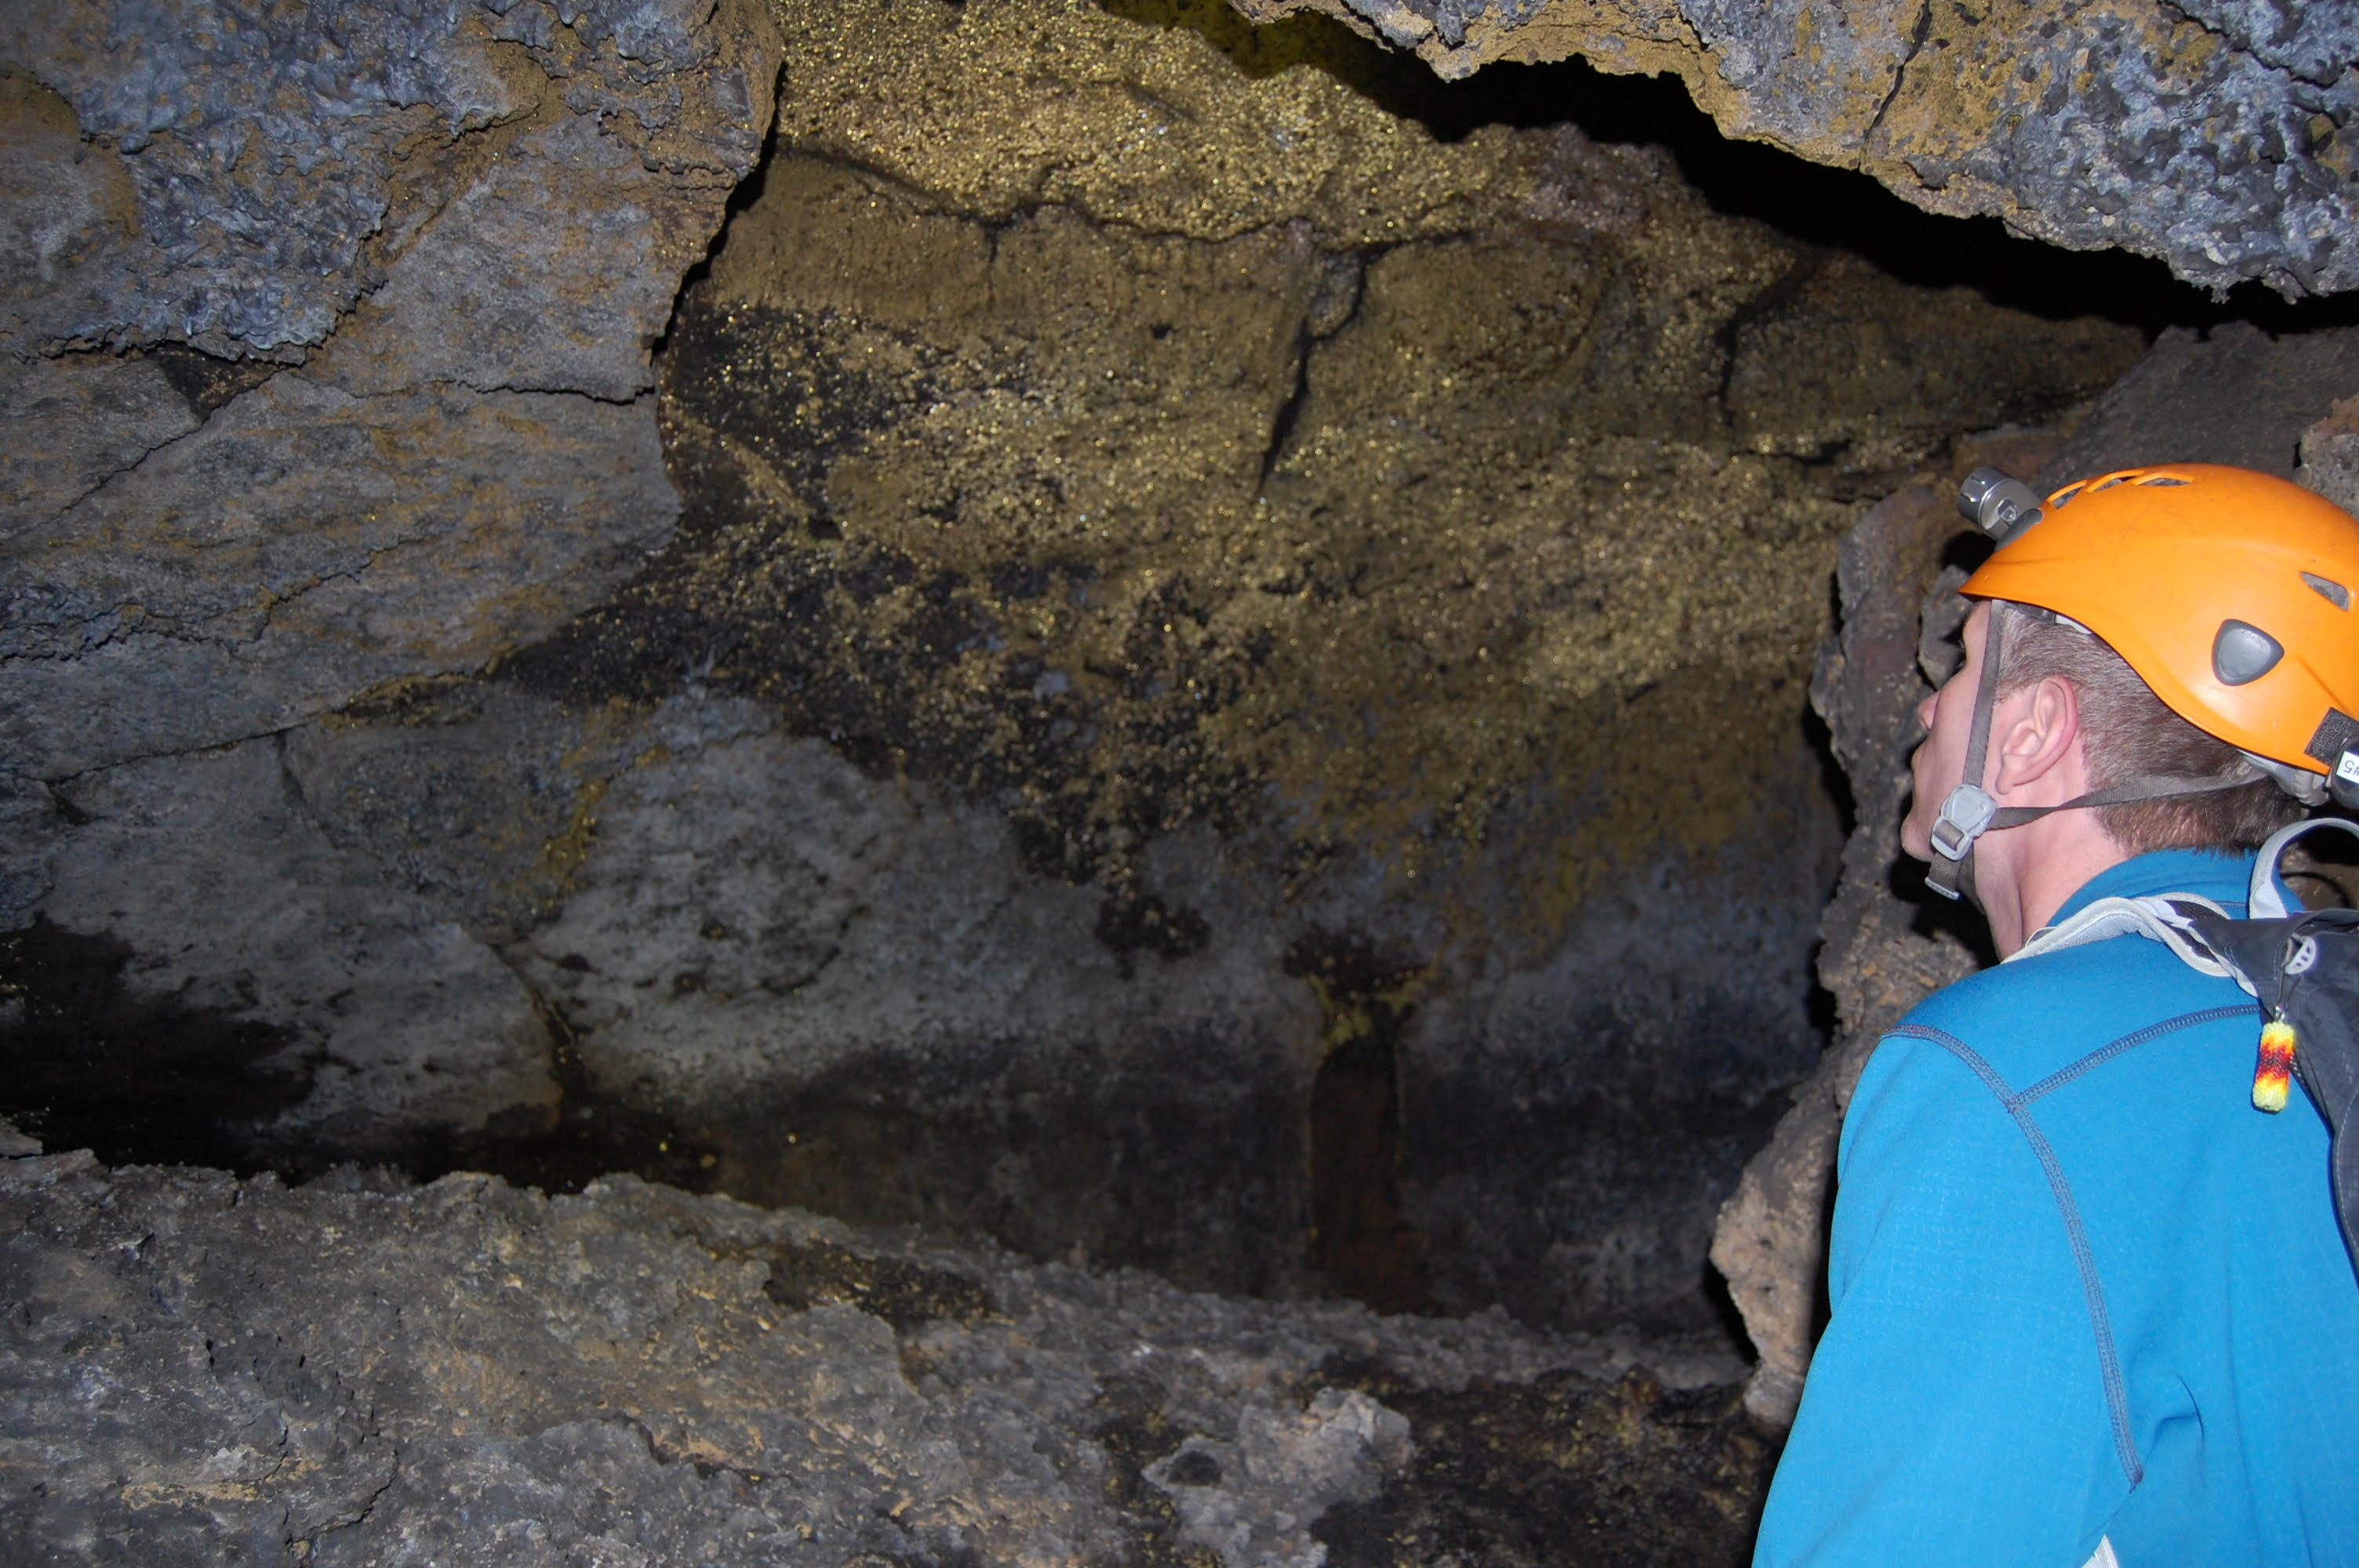
\includegraphics[width=100mm]{Interview_Figure_052}
	\centering
	\caption{Michael P. Oman-Reagan in a cave looking at golden microbial life (Lava Beds National Monument) \href{<https://www.smithsonianmag.com/travel/how-bacteria-make-underground-cave-shine-gold-and-why-nasa-wants-study-them-180955670/>}{which has been studied by astrobiologists} as an analogue for life on other worlds.
		{\normalfont\scriptsize \\ \copyright\ Michael P. Oman-Reagan, image used with permission
	}}
	\label{Interview_Figure_052}
\end{figure}

\end{labeling}

\IJSRAseparator

\IJSRAsection{Concluding thoughts}

It is inevitable that the human species will continue to expand its influence beyond planet Earth. An exciting reality, but one which should also prompt us to reflect on the present and possible futures of our relationship with space. This has, of course, long been the province of science fiction. But the importance for critical consideration right now cannot be overstated. This forum clearly indicates a variety of challenges that need be contended with, but which are not insurmountable: access to opportunity and education, uncertainty and risk and biological constraints in space exploration and potential settlements, threats to heritage, private versus public interest, support for science.

Continuing research and dialogue on these issues is essential in informing and guiding the next steps. Archaeologists, anthropologists, sociologists and other human scientists have a great role in developing understandings. Archaeology, especially, is as much about present and future concerns as it is about those past. We should be ever aware that time will not stop with us, that our actions and inactions have very real consequences, and that we have the ethical responsibility to be stewards for those lives yet to be lived.

Space anthropology and space archaeology are already productive areas of research, relevant to our presents and futures, drawing on our pasts and presents. The greatest contribution that the field can make right now is informing on policies and projects that aim to expand human activity in space. While the prospects of space exploration are beyond exciting, we need to think critically about how to make space accessible to all by asking difficult questions and learning from our collective history and heritage.

\IJSRAsection{Acknowledgements}

Thank you again to Dr.~Alice Gorman, Dr.~Cameron M. Smith, Dr. Jim Pass, Keirsten Snover, and Michael P. Oman-Reagan for their essential and insightful contributions. A chat with Keirsten Snover jump-started the idea for this forum. And thank you to Devin Ward for her comments on a previous draft that enhanced the introduction.

\IJSRAclosing
